
\section{Results}

The current results section follows the same
format used previously in this thesis;
I first present analyses of participants' responses,
followed by measures of conflict on trials where a particular response was given,
then the cursor transition probabilities,
and finally the time course data.
Each of these analyses is broken into three sections.
First, I investigated what happens on trials where both cues conflict.
Then, I tested the effect of descriptions on base rate-driven reasoning.

There were three kinds of trial in which
participants could use base rate information in this task:
trials where both the base rate and the description cued the same response
(i.e. the description agreed with the base rate),
trials where the base rate provided the only useful information
(the description was uninformative),
and trials where the description cued the opposite response
(the description disagreed with the base rate).
Most dual process theories would predict that descriptions,
being more easily and readily processed,
should interfere with base rate-based reasoning.

I also test the effect of base rates on description-cued reasoning.
There were also three types of trial where
participants could rely on the description:
trials where the description and the base rate cued the same response
(i.e. the base rate agreed with the description)
trials where only the description was useful
(the base rate was uninformative; 500:500),
and trials where the base rate cued the opposite response
(the base rate disagreed with the description).

Analyses were conducted using multilevel models,
with random intercepts for each participant, and for each problem,
unless otherwise stated.
As before, log-linear models were used for the latency data
(reading time, movement initiation time, and response time),
and logistic models for analysis of participants' responses,
and the transition probability analysis.

\subsection{Responses}

Table~\ref{tab:exp5_responses} shows the proportion of responses
consistent with each cue in each condition.
When the cues disagreed, participants selected
the description-cued response on 80.4\% of trials,
and the base rate-cued response on 19.6\%,
a statistically significant difference (z = 5.958, p < .0001).


\begin{table}[h]
  \centering
  \caption[Participants' responses, Experiment 5.]{
    Responses consistent with each cue, according to whether the
    other cue agreed with it, is uninformative, or disagreed with it, in Experiment 5.
    \label{tab:exp5_responses}
  }
  \begin{tabular}{l R{2.5cm} l l R{2.5cm}}
    \toprule
    Description   & Base rate responses & & Base rate     & Description responses\\
    \cline{1-2}
    \cline{4-5}
    Agreed        & 94.4\%              & & Agreed        & 94.4\%\\
    Uninformative & 69.4\%              & & Uninformative & 93.6\%\\
    Disagreed     & 19.6\%              & & Disagreed     & 80.4\%\\
    \bottomrule
  \end{tabular}
\end{table}

\subsubsection{Effect of descriptions on base rate choices}


Descriptions had a significant main effect on
the probability of participants' giving the base rate-cued response
($\chi^2$ = 741.6, DF = 2%
\footnote{
  Recall from Chapter 2 that Chi-squared tests
  are used in place of ANOVA F tests
  for mixed models analysis ---
  a significant chi-squared test denotes
  a significant main effect of condition here.
  }, p < .0001).
Participants were significantly more likely\footnotemark
to give the base rate cued response when
the base rate and description agreed (94.4\% of trials)
than when the description was uninformative (69.4\%)
or when the description disagreed with the base rate (19.6\%)
They were also significantly more likely to do so
when the description was uninformative
than when the description disagreed
(z's > 8, p's < .0001).

\footnotetext{All post-hoc comparisons report
  Tukey adjusted p values and confidence intervals.}

Figure~\ref{fig:exp5_br_acc} plots the number of 
base rate cued responses given by each participant, by condition,
and indicates that these effects seem to be operate consistently
across all participants, rather than being driven
by a subset of participants who are influenced by the description.
Of the 50 participants, 49 were less likely 
to give the base rate cued response
when base rates and descriptions disagreed than when they agreed,
and 1 always gave the base rate cued response.

\begin{figure}[ht]
  \centering
  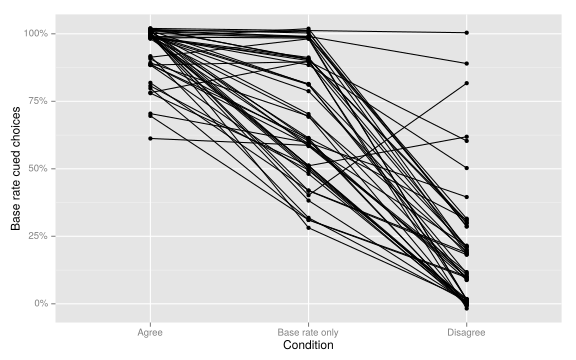
\includegraphics[width=.6\textwidth]{imgs/exp5_br_acc.pdf}
  \caption[Individual differences in the effect of descriptions
  on participants' responses, Experiment 5.]{
    Number of base rate responses per condition, by participant, in Experiment 5.
    \label{fig:exp5_br_acc} }
\end{figure}

\subsubsection{Effect of base rates on description choices}


Base rates had a significant main effect on
the number of description-cued responses given
($\chi^2$  = 67.7, DF = 2, p < .0001).
Pairwise comparisons showed that participants were
less likely to give the description-cued response
when the base rate disagreed with the description (80.4\%)
than when it agreed (94.4\%;
$e^{\beta}$ = 0.20, CI = [0.12, 0.36], z = 6.655, p < .0001)
or when the base rate was uninformative (93.6\%;
$e^{\beta}$ = 0.24, CI = [0.14, 0.42], z = 6.128, p < .0001).
There was no difference between trials in which the base rate agreed
and those where the base rate was uninformative (z < .3, p > .7),
with both conditions close to ceiling.
Therefore, participants were at least in some way
sensitive to the base rate information, and in a minority of cases
relied on it instead of the description when the two conflicted.

Once again, it is useful to investigate individual differences in this effect.
The left panel of Figure~\ref{fig:exp5_description_acc} shows
the proportion of description-cued responses given by each participant by condition.
This shows three participants who were substantially less likely
to give the description-cued response when the base rate disagreed with it.
The right panel shows the difference, for each participant,
in the number of description-cued responses given
from when the base rate agreed to when it disagreed.
This shows that, along with the 
three participants who showed a substantial change,
most participants showed a moderate effect in the same direction:
they were slightly less likely to select
the description-cued response when the base rate disagreed with it,
suggesting that base rates had some effect on the majority of participants.
Out of 50 participants, 28 were less likely
to select the description-cued response when the base rate disagreed,
13 were equally likely to do so (including 10 who always gave this response),
and 9 were actually more likely to select the description-cued response
when the description disagreed.

\begin{figure}[ht]
  \centering
  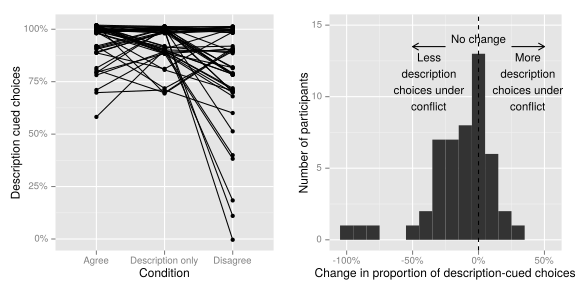
\includegraphics[width=\figurewidth]{imgs/exp5_description_acc.pdf}
  \caption[Individual differences in the effect of base rates
  on participants' responses, Experiment 5.]{
    \label{fig:exp5_description_acc}
    Left: Proportion of base rate-cued responses given in each condition,
    by participant.
    Right: Difference in the proportion of description-cued responses given
    by each participant between when the base rate agreed and disagreed with
    the description. Values below 0 indicate a participant was less likely
    to select the description-cued response when it conflicted with the base rate
    than when it agreed.
  }
\end{figure}

